% !TeX program = lualatex
\documentclass[11pt,a4paper]{article}
\usepackage{szzmaterial}
\usepackage{tikz}
\usetikzlibrary{automata,positioning,arrows.meta,calc,fit,backgrounds,shapes.geometric}
\setlist[enumerate]{nosep,leftmargin=2.1em}
\setlist[itemize]{nosep,leftmargin=1.8em}

% Vzhled automatů (sjednocený pro celý okruh)
\tikzset{
  aut/.style={->,>=Stealth,shorten >=1pt,auto,node distance=2.7cm,on grid,
    every state/.style={draw=blue!55!black,fill=blue!7,thick,minimum size=9mm,inner sep=1pt}},
}

\szztitul{Automaty a jazyky}{I1}{NTIN071 (Automaty a gramatiky)}

\begin{document}
\maketitle
\tableofcontents
\bigskip

\section*{Úvod}
\addcontentsline{toc}{section}{Úvod}

Tento materiál pokrývá okruh \textbf{I1 -- Automaty a jazyky} (předmět NTIN071 \emph{Automaty a gramatiky}). Výklad stojí na dvou zdrojích z MFF UK na úrovni kurzu pro informatiky: na \emph{slidech k~přednášce M.~Vomlelové}, z nichž bereme přesný rozsah, značení a konvence NTIN071, a na souvislém textu M.~Mareše \emph{Úvod do automatů}, o který se opíráme u prózy, intuice a důkazů u regulárních jazyků, bezkontextových gramatik a Turingových strojů. Značení a hloubka odpovídají kurzu, ne obecné teorii vyčíslitelnosti.

\noindent\textbf{Role důkazů.} Požadavky okruhu kladou důraz na \emph{konstrukce}: navrhnout konečný automat, bezkontextovou gramatiku nebo zásobníkový automat pro zadaný jazyk, provést standardní převod (podmnožinová konstrukce, gramatika $\leftrightarrow$ automat, gramatika $\to$ zásobníkový automat) a zařadit konkrétní jazyk do Chomského hierarchie. Pojmenované věty proto uvádíme se zněním, intuicí a u klíčových převodů s \emph{konstrukcí}, kterou je dobré umět provést na konkrétním vstupu. Plné formální důkazy (Kleeneho věta, ekvivalence modelů, nerozhodnutelnost) uvádíme jen v náčrtu a označujeme jako \emph{nepovinné}; podstatné je porozumět jejich myšlence. Do výkladu je zařazeno všech sedm reálných otázek SZZ k~okruhu z~let 2023--2026 jako řešené příklady; jsou i v~samostatném dokumentu \emph{Příklady otázek}. Použité zdroje jsou uvedeny na konci.

\medskip
\noindent\textbf{Značení.} \emph{Abeceda} $\Sigma$ je konečná neprázdná množina \emph{znaků}. \emph{Slovo} (řetězec) je konečná posloupnost znaků; množinu všech slov nad $\Sigma$ značíme $\Sigma^*$, \emph{prázdné slovo} (délky $0$) značíme $\lambda$ (některé texty píší $\varepsilon$). Délka slova $w$ je $|w|$, počet výskytů znaku $a$ ve slově je $|w|_a$. \emph{Zřetězení} slov $u,v$ píšeme $uv$, mocninu $w^k$, otočení $w^R$. Slovo $u$ je \emph{prefix} (\emph{sufix}) slova $w$, je-li $w=uv$ (resp.\ $w=vu$) pro nějaké $v$; je \emph{podslovem} (vždy souvislým, tj.\ faktorem), je-li $w=xuy$ pro nějaká $x,y$. \emph{Jazyk} je libovolná podmnožina $\Sigma^*$. Proměnné (neterminály) gramatik píšeme velkými písmeny $A,B,S$, terminály malými $a,b$; $\mathcal P$ je množina pravidel. Potenční množinu množiny stavů značíme $2^Q$, její konečné podmnožiny $\mathcal P_{\mathrm{FIN}}(\cdot)$. Třídy jazyků Chomského hierarchie značíme $\mathcal L_3\subset\mathcal L_2\subset\mathcal L_1\subset\mathcal L_0$ (regulární, bezkontextové, kontextové, rekurzivně spočetné).

% ============================================================
\section{Regulární jazyky (gramatiky, DFA/NFA, regulární výrazy)}

Regulární jazyky jsou nejmenší a nejlépe ovladatelná třída. Popíšeme je čtyřmi navzájem ekvivalentními způsoby: \emph{deterministickým} a \emph{nedeterministickým konečným automatem}, \emph{regulárním výrazem} a \emph{regulární (pravou lineární) gramatikou}. Že jde skutečně o tutéž třídu, je obsahem Kleeneho věty a převodů, které tvoří jádro této sekce.

\subsection{Deterministický konečný automat (DFA)}

\begin{definice}[Deterministický konečný automat]
\emph{Deterministický konečný automat} (DFA) je pětice $A=(Q,\Sigma,\delta,q_0,F)$, kde
\begin{itemize}
  \item $Q$ je konečná neprázdná množina \emph{stavů},
  \item $\Sigma$ je konečná neprázdná \emph{vstupní abeceda},
  \item $\delta\colon Q\times\Sigma\to Q$ je \emph{přechodová funkce},
  \item $q_0\in Q$ je \emph{počáteční stav},
  \item $F\subseteq Q$ je množina \emph{přijímajících} (koncových) stavů.
\end{itemize}
\end{definice}

\begin{intuice}
Automat čte vstup zleva doprava, znak po znaku, a drží si jediný „aktuální stav`` -- konečnou paměť. Přechodová funkce říká, kam se ze stavu posunout po přečtení znaku. Po dočtení vstupu se podívá, zda skončil v přijímajícím stavu. Determinismus znamená, že z každého stavu vede pro každý znak \emph{právě jeden} přechod; výpočet je tak vstupem jednoznačně určen.
\end{intuice}

Abychom mohli mluvit o přijetí celého slova, rozšíříme $\delta$ ze znaků na slova.

\begin{definice}[Rozšířená přechodová funkce, přijímaný jazyk]
\emph{Rozšířená přechodová funkce} $\delta^*\colon Q\times\Sigma^*\to Q$ je dána induktivně:
\[ \delta^*(q,\lambda)=q,\qquad \delta^*(q,wx)=\delta\big(\delta^*(q,w),x\big)\quad(q\in Q,\ w\in\Sigma^*,\ x\in\Sigma). \]
Slovo $w$ je \emph{přijímáno}, pokud $\delta^*(q_0,w)\in F$. \emph{Jazyk přijímaný automatem} $A$ je
\[ L(A)=\{\,w\in\Sigma^*\mid \delta^*(q_0,w)\in F\,\}. \]
Jazyk $L$ je \emph{regulární}, existuje-li DFA $A$ s $L=L(A)$.
\end{definice}

V obrázcích kreslíme stav jako kroužek, počáteční stav značíme šipkou „odnikud``, přijímající stavy dvojitým okrajem. Hrana z $p$ do $q$ označená $x$ znamená $\delta(p,x)=q$.

\begin{center}
\scalebox{1.2}{%
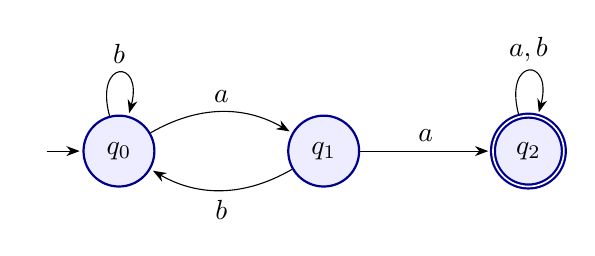
\begin{tikzpicture}[aut,node distance=2.6cm]
  \node[state,initial,initial text={}] (q0) {$q_0$};
  \node[state] (q1) [right=of q0] {$q_1$};
  \node[state,accepting] (q2) [right=of q1] {$q_2$};
  \path (q0) edge[loop above] node{$b$} (q0)
        (q0) edge[bend left] node{$a$} (q1)
        (q1) edge[bend left] node{$b$} (q0)
        (q1) edge node{$a$} (q2)
        (q2) edge[loop above] node{$a,b$} (q2);
\end{tikzpicture}%
}
\end{center}
\obrpopis{obecné schéma DFA (konvence kreslení) nad $\Sigma=\{a,b\}$. \textbf{Kroužek} $=$ stav; \textbf{vstupní šipka} „odnikud`` $=$ počáteční stav ($q_0$); \textbf{dvojitý kroužek} $=$ přijímající stav ($q_2$); \textbf{šipka} mezi stavy s návěštím $x$ $=$ přechod $\delta(p,x)=q$. U DFA vede z \emph{každého} stavu \emph{právě jeden} přechod na \emph{každý} symbol abecedy (každý stav je „totální``): zde $q_0$ má hranu na $a$ i na $b$, $q_1$ má hranu na $a$ i na $b$ a $q_2$ má smyčku $a,b$ (jeden přechod značící obě hodnoty). Výpočet je proto vstupem jednoznačně určen.}

\begin{center}
\scalebox{1.2}{%
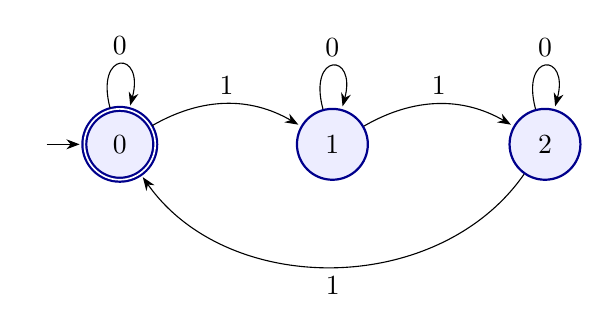
\begin{tikzpicture}[aut]
  \node[state,initial,initial text={},accepting] (s0) {$0$};
  \node[state] (s1) [right=of s0] {$1$};
  \node[state] (s2) [right=of s1] {$2$};
  \path (s0) edge[loop above] node{$0$} (s0)
        (s1) edge[loop above] node{$0$} (s1)
        (s2) edge[loop above] node{$0$} (s2)
        (s0) edge[bend left] node{$1$} (s1)
        (s1) edge[bend left] node{$1$} (s2)
        (s2) edge[bend left=55] node{$1$} (s0);
\end{tikzpicture}%
}
\end{center}
\obrpopis{DFA nad $\Sigma=\{0,1\}$ přijímající $\{w\mid |w|_1\equiv 0\pmod 3\}$, tj.\ slova s počtem jedniček dělitelným třemi. Stav $i$ znamená „dosud přečteno $i$ jedniček mod~$3$``; znak $0$ zbytek nemění (smyčky), znak $1$ zvyšuje o~$1$. Počáteční i jediný přijímající stav je $0$. Např.\ při čtení $0110$ projdeme stavy $0\to0\to1\to2\to2$ (poslední $0$ stav nemění), takže $\delta^*(0,0110)=2\notin F$ a slovo $0110$ přijato \emph{není} ($|0110|_1=2$).}

\begin{poznamka}
Determinismus dává okamžitě \textbf{rozhodovací algoritmus}: slovo délky $n$ otestujeme v čase $O(n)$ prostým odsimulováním přechodů. To je hlavní praktická přednost konečných automatů (vyhledávání vzorů, lexikální analýza).
\end{poznamka}

\begin{priklad}[SZZ léto 2025 č.~1: Deterministické konečné automaty]
\szzotazka{léto 2025}{1}{Deterministické konečné automaty (jazyk DFA, rozšířená přechodová funkce)}\par
\textbf{Zadání.}\par
\begin{enumerate}
  \item Uveďte definici jazyka $L(A)$ přijímaného daným DFA $A=(Q,\Sigma,\delta,q_0,F)$ včetně definice rozšířené přechodové funkce $\delta^*$.
  \item Nechť $S\subseteq\Sigma^*$ je neprázdná konečná množina slov, $Q$ je množina všech prefixů slov z $S$ (vč.\ $\lambda$ a slov z $S$) a $A=(Q,\Sigma,\delta,\lambda,S)$. Definujte $\delta$ tak, aby $A$ přijímal jazyk $\{w\mid w$ obsahuje nějaké $s\in S$ jako podslovo$\}$.
  \item Sestrojte DFA přijímající $\{w\in\{0,1\}^*\mid w$ obsahuje $010$ nebo končí na $10\}$.
\end{enumerate}

\smallskip
\textbf{Řešení.}\par
\textbf{(1)} Přesně definice výše: $\delta^*(q,\lambda)=q$, $\delta^*(q,wx)=\delta(\delta^*(q,w),x)$ a $L(A)=\{w\mid\delta^*(q_0,w)\in F\}$.

\textbf{(2)} Stav je nejdelší sufix dosud přečteného slova, který je v $Q$ (tj.\ je prefixem nějakého $s\in S$ nebo přímo nějakým $s$). Jakmile se objeví celé $s\in S$, zůstaneme v něm napořád (podslovo už ze slova nezmizí). Pro $w\in Q$, $x\in\Sigma$:
\[ \delta(w,x)=\begin{cases}
  w, & w\in S\ \text{(absorbující -- podslovo už nalezeno)},\\
  s, & w\notin S\ \text{a $wx$ končí na nějaké $s\in S$ (vezmi nejkratší)},\\
  v, & \text{jinak; $v$ = nejdelší sufix slova $wx$ ležící v $Q$.}
\end{cases} \]
Přijímající stavy jsou $F=S$. Indukcí podle $|w|$: po přečtení $w$ je automat ve stavu „nejdelší sufix $w$, který je v $Q$``, případně v absorbujícím $s$, pokud $w$ obsahuje nějaké $s\in S$.

\textbf{(3)} Zde je $S=\{010,10\}$, ale s tím rozdílem, že „$010$`` se hledá jako \emph{podslovo} (absorbující), kdežto „$10$`` se vyžaduje jen \emph{na konci}. Stavy odpovídají relevantním sufixům $Q=\{\lambda,0,1,01,10,010\}$; jediný absorbující přijímající stav je $010$, druhý přijímající stav $10$ je „obyčejný`` (značí, že právě teď slovo končí na $10$, ale ještě jsme neviděli $010$). Přechodová funkce:
\begin{center}\small
\begin{tabular}{c|cc}
\toprule
stav & $\delta(\cdot,0)$ & $\delta(\cdot,1)$\\
\midrule
$\lambda$ & $0$ & $1$\\
$0$ & $0$ & $01$\\
$1$ & $10$ & $1$\\
$01$ & $010$ & $1$\\
$\mathbf{10}$ & $0$ & $01$\\
$\mathbf{010}$ & $010$ & $010$\\
\bottomrule
\end{tabular}
\end{center}
Počáteční stav $\lambda$, přijímající $F=\{10,010\}$. Že automat přijímá přesně $\{w\mid w$ obsahuje $010$ nebo končí na $10\}$, jsme \emph{ověřili vyčerpáním všech slov do délky $12$} (Python). Klíč: ze stavu $010$ se už nedostaneme (podslovo nalezeno), kdežto ze stavu $10$ po přečtení dalšího znaku „spadneme`` (na $0$ do stavu $0$, na $1$ do $01$), takže přijetí přes $10$ vyžaduje skutečný konec na $10$.\par
\emph{Stavový diagram (oříznutý z originálu) je v} \texttt{priklady/}.
\end{priklad}

\subsection{Nedeterministický konečný automat (NFA)}

Při konstrukci je často pohodlnější dovolit z jednoho stavu \emph{více} (nebo \emph{žádný}) přechod pro tentýž znak a „uhodnout`` správnou cestu. To vede k nedeterminismu.

\begin{definice}[Nedeterministický konečný automat]
\emph{Nedeterministický konečný automat} (NFA) je pětice $A=(Q,\Sigma,\delta,Q_0,F)$, kde $\delta\colon Q\times\Sigma\to 2^Q$ přiřadí dvojici (stav, znak) \emph{množinu} možných následujících stavů, $Q_0\subseteq Q$ je množina počátečních stavů a ostatní složky jsou jako u DFA. \emph{Výpočet} je libovolná posloupnost stavů $s_0,\dots,s_{|w|}$ s $s_0\in Q_0$ a $s_{i+1}\in\delta(s_i,w[i])$. Slovo je \emph{přijato}, existuje-li \emph{aspoň jeden} výpočet končící v $F$.
\end{definice}

\begin{intuice}
NFA přijme slovo, pokud \emph{existuje} úspěšná cesta -- jako bychom směli vždy zvolit tu šťastnou možnost (nebo paralelně sledovat všechny). To usnadňuje návrh (jeden „hlídač`` na každou alternativu), ale nezvyšuje sílu: nedeterminismus jde vždy odstranit.
\end{intuice}

\begin{center}
% DFA (vlevo): z q0 právě jeden přechod na a
\scalebox{1.2}{%
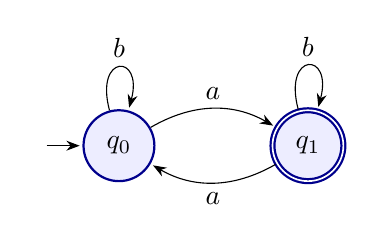
\begin{tikzpicture}[aut,node distance=2.4cm]
  \node[state,initial,initial text={}] (p0) {$q_0$};
  \node[state,accepting] (p1) [right=of p0] {$q_1$};
  \path (p0) edge[loop above] node{$b$} (p0)
        (p0) edge[bend left] node{$a$} (p1)
        (p1) edge[bend left] node{$a$} (p0)
        (p1) edge[loop above] node{$b$} (p1);
\end{tikzpicture}%
}
\hspace{1.4cm}
% NFA (vpravo): z q0 dva přechody na a + lambda-prechod
\scalebox{1.2}{%
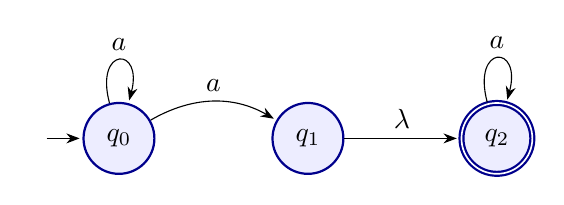
\begin{tikzpicture}[aut,node distance=2.4cm]
  \node[state,initial,initial text={}] (r0) {$q_0$};
  \node[state] (r1) [right=of r0] {$q_1$};
  \node[state,accepting] (r2) [right=of r1] {$q_2$};
  \path (r0) edge[loop above] node{$a$} (r0)
        (r0) edge[bend left] node{$a$} (r1)
        (r1) edge node{$\lambda$} (r2)
        (r2) edge[loop above] node{$a$} (r2);
\end{tikzpicture}%
}
\end{center}
\obrpopis{DFA versus NFA (nedeterminismus). \emph{Vlevo DFA}: z každého stavu vede na každý symbol \emph{právě jeden} přechod (z $q_0$ vede na $a$ jediná hrana do $q_1$), výpočet je jednoznačný. \emph{Vpravo NFA}: ze stavu $q_0$ vedou na týž symbol $a$ \emph{dva} přechody (smyčka do $q_0$ a hrana do $q_1$) -- automat si „vybírá``; navíc je tu $\lambda$-přechod $q_1\to q_2$, který \emph{nečte žádný symbol}. NFA tedy z jednoho stavu může mít na symbol více přechodů (nebo žádný) a slovo \emph{přijme, pokud existuje aspoň jedna} úspěšná větev výpočtu končící v přijímajícím stavu.}

\begin{veta}[Podmnožinová konstrukce]
Ke každému NFA $A$ existuje DFA $A'$ s $L(A')=L(A)$. Tudíž jazyk je rozpoznatelný NFA právě tehdy, je-li regulární.
\end{veta}

\begin{proof}[Důkaz \textnormal{(nepovinný -- konstrukce)}]
Stav DFA bude celá \emph{množina} stavů, v nichž se NFA může nacházet. Položíme $A'=(2^Q,\Sigma,\delta',Q_0,F')$, kde
\[ \delta'(S,x)=\bigcup_{s\in S}\delta(s,x),\qquad F'=\{S\subseteq Q\mid S\cap F\neq\emptyset\}. \]
Indukcí podle délky slova platí $\delta'^*(Q_0,w)=\{\,\delta\text{-dosažitelné stavy NFA po }w\,\}$, takže $A'$ přijme $w$ právě když nějaký výpočet NFA končí v $F$. Stačí vzít \emph{dosažitelné} stavy (typicky jich je málo, ne všech $2^{|Q|}$).
\end{proof}

\begin{poznamka}[$\lambda$-přechody]
Při skládání automatů (sjednocení, zřetězení, iterace) se hodí přechody, které \emph{nečtou žádný znak} -- tzv.\ \emph{$\lambda$-přechody}. \emph{$\lambda$-NFA} má $\delta\colon Q\times(\Sigma\cup\{\lambda\})\to 2^Q$. I ty jdou odstranit: stavy zachováme a přechodovou funkci i počáteční stavy „uzavřeme`` na $\lambda$-okolí ($\lambda$-uzávěr stavu = množina stavů dosažitelných po samých $\lambda$-hranách). Proto i $\lambda$-NFA rozpoznávají právě regulární jazyky.
\end{poznamka}

Následující reálná otázka prochází celý okruh „regulární výraz $\to$ NFA $\to$ DFA $\to$ doplněk`` a je dobrým souhrnem této a předchozí podsekce.

\begin{priklad}[SZZ podzim 2024 č.~1: Doplněk regulárního výrazu]
\szzotazka{podzim 2024}{1}{Doplněk regulárního výrazu (NFA/DFA, podmnožinová konstrukce, doplněk)}\par
\textbf{Zadání.}\par
Pro $R=((a+b)(a+b))^*ab$ nad $\Sigma=\{a,b\}$ a $L=L(R)$:
\begin{enumerate}
  \item Sestrojte (co nejmenší) NFA $A$ pro $L$.
  \item Podmnožinovou konstrukcí převeďte $A$ na DFA $B$.
  \item Z $B$ sestrojte DFA $C$ pro \emph{doplněk} $\overline L$.
\end{enumerate}

\smallskip
\textbf{Řešení.}\par
Výraz $R$ popisuje slova \emph{sudé délky končící na $ab$} (před závěrečným $ab$ stojí libovolný \emph{sudý} počet znaků).

\textbf{(1) NFA $A$.} Stavy $\{q_0,q_1,q_2,q_F\}$: $q_0$ je „začátek dvojice / odhad konce``, $q_1$ „uprostřed dvojice``, $q_2$ „uhodli jsme závěrečné $a$``, $q_F$ přijímá. Nedeterministicky buď spotřebujeme dvojici $(a{+}b)(a{+}b)$ a vrátíme se do $q_0$, nebo zahájíme závěrečné $ab$:
\[ \delta(q_0,a)=\{q_1,q_2\},\quad \delta(q_0,b)=\{q_1\},\quad \delta(q_1,a)=\delta(q_1,b)=\{q_0\},\quad \delta(q_2,b)=\{q_F\}. \]

\textbf{(2) DFA $B$ (podmnožinová konstrukce).} Dosažitelné množiny stavů (počáteční $\{q_0\}$):
\begin{center}\small
\begin{tabular}{c|cc}
\toprule
stav $B$ & $a$ & $b$\\
\midrule
$\{q_0\}$ & $\{q_1,q_2\}$ & $\{q_1\}$\\
$\{q_1,q_2\}$ & $\{q_0\}$ & $\{q_0,q_F\}$\\
$\{q_1\}$ & $\{q_0\}$ & $\{q_0\}$\\
$\{q_0,q_F\}^{*}$ & $\{q_1,q_2\}$ & $\{q_1\}$\\
\bottomrule
\end{tabular}
\end{center}
Jediný přijímající stav je $\{q_0,q_F\}$ (obsahuje $q_F$). Přechodová funkce je \emph{totální} (každý stav má oba přechody), takže nepřibyl žádný stav „žumpa``.

\textbf{(3) DFA $C$ pro doplněk.} U DFA s \emph{totální} $\delta$ stačí prohodit přijímající a nepřijímající stavy: $C$ má tytéž stavy a přechody jako $B$, ale $F_C=\{\{q_0\},\{q_1,q_2\},\{q_1\}\}$. (Kdyby $\delta$ totální nebyla, museli bychom napřed doplnit žumpu, jinak by doplněk vynechal slova, na kterých $B$ „uvízne``.)
\begin{center}
% NFA A
\scalebox{1.2}{%
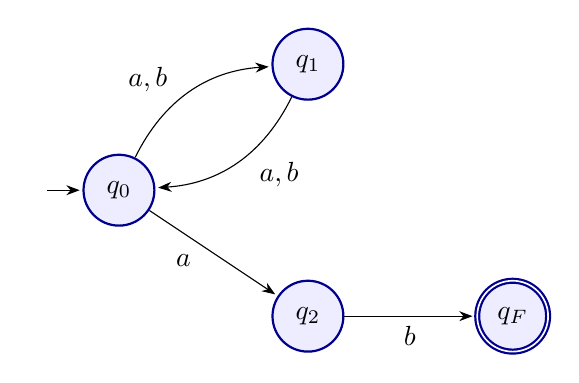
\begin{tikzpicture}[aut,node distance=2.4cm]
  \node[state,initial,initial text={}] (q0) {$q_0$};
  \node[state] (q1) [above right=1.6cm and 2.4cm of q0] {$q_1$};
  \node[state] (q2) [below right=1.6cm and 2.4cm of q0] {$q_2$};
  \node[state,accepting] (qF) [right=2.6cm of q2] {$q_F$};
  \path (q0) edge[bend left] node[pos=.4]{$a,b$} (q1)
        (q1) edge[bend left] node[pos=.4]{$a,b$} (q0)
        (q0) edge node[swap,pos=.4]{$a$} (q2)
        (q2) edge node[swap]{$b$} (qF);
\end{tikzpicture}%
}
\hspace{0.6cm}
% DFA B
\scalebox{1.2}{%
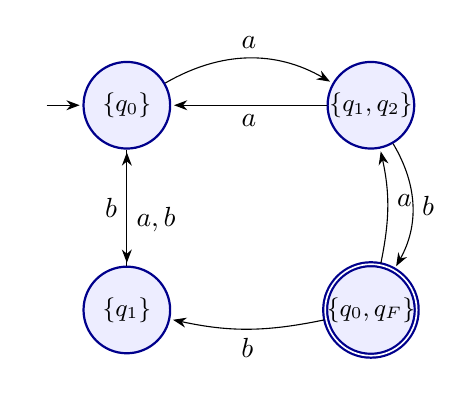
\begin{tikzpicture}[aut,node distance=2.9cm,
   every state/.style={draw=blue!55!black,fill=blue!7,thick,minimum size=11mm,inner sep=0pt,font=\small}]
  \node[state,initial,initial text={}] (A) {$\{q_0\}$};
  \node[state] (B) [right=3.1cm of A] {$\{q_1,q_2\}$};
  \node[state] (D) [below=2.6cm of A] {$\{q_1\}$};
  \node[state,accepting] (C) [below=2.6cm of B] {$\{q_0,q_F\}$};
  \path (A) edge[bend left] node{$a$} (B)
        (A) edge node[swap]{$b$} (D)
        (B) edge[bend left] node{$b$} (C)
        (B) edge node{$a$} (A)
        (D) edge node[swap,pos=.4]{$a,b$} (A)
        (C) edge[bend right=12] node[swap,pos=.55]{$a$} (B)
        (C) edge[bend left=12] node[pos=.5]{$b$} (D);
\end{tikzpicture}%
}
\end{center}
\obrpopis{vlevo nejmenší NFA $A$ pro $((a+b)(a+b))^*ab$ ($4$ stavy; méně jich být nemůže: pro dvojice $(x_i,y_i)\in\{(\lambda,ab),(a,b),(ab,\lambda),(b,aab)\}$ je vždy $x_iy_i\in L$, ale pro $i\neq j$ do $L$ nepatří $x_iy_j$ nebo $x_jy_i$, takže stavy po přečtení $x_i$ na přijímajících výpočtech musí být navzájem různé), vpravo DFA $B$ z podmnožinové konstrukce ($4$ dosažitelné stavy, $\delta$ totální). DFA $C$ pro $\overline L$ vznikne z $B$ záměnou přijímajících stavů (přijímající budou $\{q_0\},\{q_1,q_2\},\{q_1\}$). Správnost NFA i konstrukce ověřena vyčerpáním slov do délky $10$. Diagramy všech tří automatů (oříznuté z originálu) jsou v \texttt{priklady/}.}
\end{priklad}

\subsection{Regulární výrazy a Kleeneho věta}

\begin{definice}[Regulární výraz]
\emph{Regulární výrazy} nad $\Sigma$ a jimi popsané jazyky definujeme induktivně:
\[ \emptyset\ (L=\emptyset),\quad \lambda\ (L=\{\lambda\}),\quad x\ (L=\{x\},\ x\in\Sigma), \]
a pro výrazy $X,Y$: $X+Y$ (sjednocení $L(X)\cup L(Y)$), $XY$ (zřetězení $L(X)\cdot L(Y)$), $X^*$ (iterace $L(X)^*$). Zkratky: $X^+=XX^*$, $X?=X+\lambda$.
\end{definice}

\begin{veta}[Kleeneho]
Jazyk je popsatelný regulárním výrazem právě tehdy, je-li regulární.
\end{veta}

\begin{intuice}
Směr „výraz $\Rightarrow$ regulární`` je stavebnice: pro každou operaci sestrojíme $\lambda$-NFA z dílčích automatů (viz schéma níže). Opačný směr (\emph{eliminace stavů}) z DFA postupně odstraňuje stavy a hrany ohodnocuje regulárními výrazy, až zbude jediná hrana mezi počátečním a koncovým stavem -- její ohodnocení je hledaný výraz.
\end{intuice}

\begin{center}
\scalebox{1.15}{%
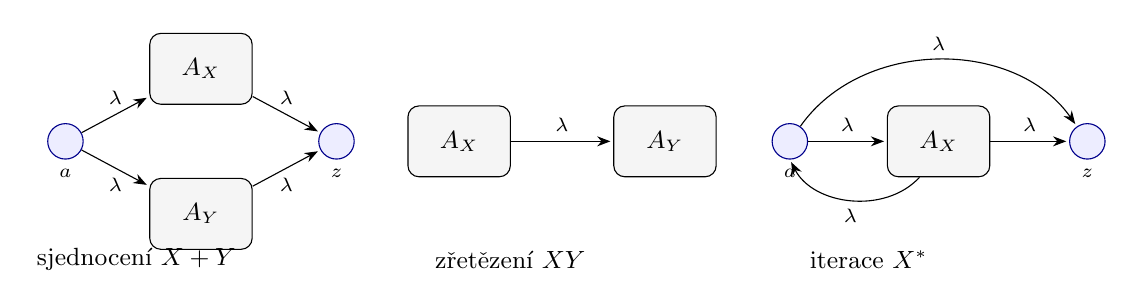
\begin{tikzpicture}[->,>=Stealth,shorten >=1pt,node distance=1.2cm,
   blk/.style={draw,rounded corners,fill=black!4,minimum width=13mm,minimum height=9mm,font=\small},
   sm/.style={circle,draw=blue!55!black,fill=blue!7,inner sep=1.2pt,minimum size=4.5mm,font=\scriptsize}]
% Sjednoceni
\begin{scope}
  \node[sm,label=below:{\scriptsize $a$}] (a) {};
  \node[blk] (X) [above right=0.3cm and 0.9cm of a] {$A_X$};
  \node[blk] (Y) [below right=0.3cm and 0.9cm of a] {$A_Y$};
  \node[sm,label=below:{\scriptsize $z$}] (z) [below right=0.3cm and 0.9cm of X] {};
  \path (a) edge node[above,font=\scriptsize]{$\lambda$} (X)
        (a) edge node[below,font=\scriptsize]{$\lambda$} (Y)
        (X) edge node[above,font=\scriptsize]{$\lambda$} (z)
        (Y) edge node[below,font=\scriptsize]{$\lambda$} (z);
  \node[font=\small] at (0.9,-1.5) {sjednocení $X+Y$};
\end{scope}
% Zretezeni
\begin{scope}[shift={(5.0,0)}]
  \node[blk] (X) {$A_X$};
  \node[blk] (Y) [right=1.3cm of X] {$A_Y$};
  \path (X) edge node[above,font=\scriptsize]{$\lambda$} (Y);
  \node[font=\small] at (0.65,-1.5) {zřetězení $XY$};
\end{scope}
% Iterace
\begin{scope}[shift={(9.2,0)}]
  \node[sm,label=below:{\scriptsize $a$}] (a) {};
  \node[blk] (X) [right=1.0cm of a] {$A_X$};
  \node[sm,label=below:{\scriptsize $z$}] (z) [right=1.0cm of X] {};
  \path (a) edge node[above,font=\scriptsize]{$\lambda$} (X)
        (X) edge node[above,font=\scriptsize]{$\lambda$} (z)
        (a) edge[bend left=55] node[above,font=\scriptsize]{$\lambda$} (z)
        (X) edge[bend left=55] node[below,font=\scriptsize]{$\lambda$} (a.south);
  \node[font=\small] at (1.0,-1.5) {iterace $X^*$};
\end{scope}
\end{tikzpicture}%
}
\end{center}
\obrpopis{Kleeneho „stavebnice`` regulárních jazyků pomocí $\lambda$-NFA. $A_X,A_Y$ jsou automaty pro $X,Y$ s jediným počátečním a jediným koncovým stavem. \emph{Sjednocení}: nový start a cíl, $\lambda$-hrany do/z obou. \emph{Zřetězení}: $\lambda$-hrana z konce $A_X$ na začátek $A_Y$. \emph{Iterace}: nový start/cíl, $\lambda$-hrany start$\to$cíl (přijetí $\lambda$), start$\to A_X$, konec~$A_X\to$start (opakování) a konec~$A_X\to$cíl.}

\begin{poznamka}
Konkrétně se \emph{eliminace stavů} provádí na \emph{GNFA} (hrany ohodnocené regulárními výrazy): automat doplníme o nový počáteční stav ($\lambda$-hrana do původního startu, bez vstupních hran) a nový koncový stav ($\lambda$-hrany ze všech koncových, bez výstupních) a pak po jednom rušíme vnitřní stavy. Odstraníme-li $q$, pro každou dvojici hran $p\to q$ a $q\to r$ přeznačíme hranu $p\to r$ na
\[ R(p,r)\;+\;R(p,q)\,R(q,q)^*\,R(q,r), \]
kde $R(q,q)$ je smyčka na $q$ (chybí-li, je $R(q,q)^*=\lambda$) a $R(p,r)$ je dosavadní přímá hrana ($\emptyset$, není-li žádná); smyčka rušeného stavu se tak promítne jako hvězdička. Např.\ pro DFA výše (počet jedniček dělitelný třemi) dá odstranění stavů $1$ a~$2$ výraz $(0+10^*10^*1)^*$, ekvivalentně $(0^*10^*10^*1)^*0^*$.
\end{poznamka}

\subsection{Regulární gramatiky (typ 3)}

Čtvrtý ekvivalentní popis je \emph{generativní}: pravidla, jimiž z počátečního symbolu „vyrobíme`` slovo.

\begin{definice}[Pravá lineární gramatika, typ 3]
\emph{Pravá lineární gramatika} (typ~3) je $G=(V,T,\mathcal P,S)$, kde $V$ jsou neterminály, $T$ terminály, $S\in V$ počáteční a $\mathcal P$ obsahuje jen pravidla tvaru $A\to wB$ a $A\to w$ ($A,B\in V$, $w\in T^*$). \emph{Derivace} přepisuje neterminály podle pravidel; jazyk $L(G)=\{w\in T^*\mid S\Rightarrow^* w\}$ je množina slov odvoditelných ze~$S$.
\end{definice}

\begin{veta}[Regulární gramatiky $=$ konečné automaty]
Třída jazyků generovaných pravými lineárními gramatikami je přesně třída regulárních jazyků.
\end{veta}

\begin{intuice}
Soulad je doslovný: \emph{neterminál $=$ stav}, \emph{pravidlo $=$ přechod}. Z DFA $A=(Q,\Sigma,\delta,q_0,F)$ uděláme gramatiku s $V=Q$, $S=q_0$ a pravidly $X\to aY$ pro $\delta(X,a)=Y$ a $X\to\lambda$ pro $X\in F$. Opačně sestrojíme $\lambda$-NFA: pravidlo $A\to a_1\cdots a_kB$ rozložíme přes nové pomocné stavy na řetěz přechodů z~$A$ do $B$ (pro $k=0$ je to $\lambda$-přechod), pravidlo $A\to a_1\cdots a_k$ vede takovým řetězem do nového koncového stavu. Každé slovo derivace (až na výsledné terminální) obsahuje právě jeden neterminál, a to úplně vpravo -- přesně jako „aktuální stav`` při čtení.
\end{intuice}

\begin{poznamka}
\emph{Levá} lineární gramatika ($A\to Bw$) generuje rovněž jen regulární jazyky (otočením). Pozor: obecná \emph{lineární} gramatika ($A\to wBv$) už umí i neregulární jazyk $\{0^n1^n\}$ -- proto patří mezi bezkontextové, ne regulární.
\end{poznamka}

\subsection{Iterační (pumpovací) lemma a uzávěrové vlastnosti}

Jak ukázat, že jazyk \emph{není} regulární? Konečný automat má konečně mnoho stavů, takže na dlouhém slově se nějaký stav musí zopakovat -- a úsek mezi opakováními lze libovolně „napumpovat``.

\begin{veta}[Iterační lemma pro regulární jazyky]
Pro každý regulární jazyk $L$ existuje $n\in\mathbb N$ tak, že každé $w\in L$ s $|w|\ge n$ lze rozložit na $w=xyz$, kde
\[ y\neq\lambda,\qquad |xy|\le n,\qquad xy^kz\in L\ \text{pro všechna } k\ge 0. \]
\end{veta}

\begin{proof}[Důkaz \textnormal{(nepovinný -- princip opakování stavu)}]
Za $n$ vezmeme počet stavů DFA pro $L$. Při čtení $w$, $|w|\ge n$, projde automat posloupností $s_0,s_1,\dots,s_{|w|}$, v níž se mezi prvními $n+1$ stavy nějaký zopakuje: $s_i=s_j$, $i<j\le n$. Pro $w=w_1\cdots w_m$ položíme $x=w_1\cdots w_i$, $y=w_{i+1}\cdots w_j$, $z=w_{j+1}\cdots w_m$. Smyčka z $s_i$ do $s_j$ čte $y$, takže ji lze projít $k$-krát (i nulakrát) se stejným koncovým stavem; proto $xy^kz\in L$.
\end{proof}

\begin{center}
\scalebox{1.2}{%
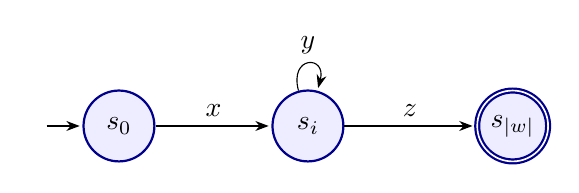
\begin{tikzpicture}[aut,node distance=2.0cm]
  \node[state,initial,initial text={}] (s0) {$s_0$};
  \node[state] (si) [right=2.4cm of s0] {$s_i$};
  \node[state,accepting] (sm) [right=2.6cm of si] {$s_{|w|}$};
  \path (s0) edge node{$x$} (si)
        (si) edge node{$z$} (sm)
        (si) edge[loop above,looseness=5] node{$y$} (si);
\end{tikzpicture}%
}
\end{center}
\obrpopis{jádro iteračního lemmatu. Po přečtení prefixu $x$ je automat ve stavu $s_i=s_j$; úsek $y$ tvoří \emph{smyčku} v tomto stavu. Smyčku lze projít libovolně-krát, proto $xy^kz\in L$ pro každé $k\ge 0$. Naopak: jazyk, který takovou „napumpovatelnost`` porušuje (např.\ $\{0^m1^m\}$ -- napumpováním $y$ z prvních nul rozbijeme rovnost počtů), \emph{není} regulární.}

\begin{intuice}
Lemma se používá jako \emph{nutná podmínka}: chceme-li dokázat neregularitu, zvolíme vhodné dlouhé slovo $w\in L$ a ukážeme, že \emph{žádný} rozklad $xyz$ s danými vlastnostmi nepřežije napumpování. Klasika: $\{0^m1^m\}$, $\{ww\mid w\in\{0,1\}^*\}$, $\{0^p\mid p$ prvočíslo$\}$.
\end{intuice}

Regulární jazyky jsou \emph{uzavřené} na všechny obvyklé operace. Nejužitečnější konstrukcí je \emph{součin automatů} pro průnik (a po malé úpravě i sjednocení).

\begin{veta}[Uzávěrové vlastnosti]
Jsou-li $X,Y$ regulární, jsou regulární i $X\cup Y$, $X\cap Y$, $\overline X=\Sigma^*\setminus X$, $X\cdot Y$, $X^*$ a $X^R$.
\end{veta}

\begin{proof}[Důkaz \textnormal{(nepovinný -- součin pro průnik)}]
Pro $X=L(A_1)$, $Y=L(A_2)$ sestrojíme \emph{součin} $A_1\times A_2$ se stavy $Q_1\times Q_2$, přechody $\delta((s_1,s_2),x)=(\delta_1(s_1,x),\delta_2(s_2,x))$, počátkem $(q_{01},q_{02})$ a $F=F_1\times F_2$. Automat běží paralelně a přijme, právě když přijmou oba: $L=X\cap Y$. Pro sjednocení vezmeme $F=(F_1\times Q_2)\cup(Q_1\times F_2)$, doplněk dá záměna $F$ za $Q\setminus F$ (u DFA s totální $\delta$), zřetězení a iterace plynou z Kleeneho stavebnice a otočení $X^R$ z~obrácení všech hran automatu (počáteční a koncové stavy si vymění role, vznikne NFA).
\end{proof}

Konstrukce DFA může být i \emph{parametrická} (automat závislý na vstupním parametru). Ukázkou je následující otázka, kde stavy nesou \emph{zbytky modulo $p$}.

\begin{priklad}[SZZ jaro 2026 č.~1: Porovnání modulárních hashů]
\szzotazka{jaro 2026}{1}{Porovnání modulárních hashů (definice DFA, konstrukce DFA)}\par
\textbf{Zadání.}\par
Pro prvočíslo $p\ge 2$ a $w\in\{0,1\}^*$ buď $h(w)=\big(\sum_{i=1}^{|w|}w_i\,2^{|w|-i}\big)\bmod p$ (hodnota binárního zápisu $w$ modulo $p$, $h(\lambda)=0$). Uvažme $L_p=\{u\#v\mid u,v\in\{0,1\}^*,\ h(u)=h(v)\}$ nad $\Sigma=\{0,1,\#\}$. (1) Definujte DFA. (2) Popište konstrukci DFA $A_p$ pro $L_p$ podle $p$. (3) Nakreslete $A_2$.

\smallskip
\textbf{Řešení.}\par
\textbf{(1)} Pětice $A=(Q,\Sigma,\delta,q_0,F)$ jako v definici výše (zde $\delta$ může být parciální -- nedefinované přechody vedou do implicitní žumpy).

\textbf{(2)} Čteme-li binární číslo zleva, platí Hornerovo schéma: přečtením dalšího bitu $b$ se zbytek $i$ změní na $(2i+b)\bmod p$. Stav si pamatuje zbytek právě čtené části:
\begin{itemize}
  \item $Q=[p]\cup[p]\times[p]$, kde $[p]=\{0,\dots,p-1\}$. Stav $i$ znamená „čteme $u$, zatím $h(u')=i$``; stav $(i,j)$ znamená „už jsme přečetli $\#$, $h(u)=i$ a zatím $h(v')=j$``.
  \item $q_0=0$, $F=\{(i,i)\mid i\in[p]\}$.
  \item $\delta(i,0)=2i\bmod p$, $\ \delta(i,1)=(2i+1)\bmod p$, $\ \delta(i,\#)=(i,0)$;
  \item $\delta((i,j),0)=(i,2j\bmod p)$, $\ \delta((i,j),1)=(i,(2j+1)\bmod p)$.
\end{itemize}
Druhé $\#$ nemá přechod -- vede do žumpy, takže $A_p$ přijme jen slova tvaru $u\#v$ s $h(u)=h(v)$. Správnost ověřena vyčerpáním slov do délky $8$ nad $\{0,1,\#\}$ pro $p=2$, $3$ a~$5$ (Python).

\textbf{(3)} Pro $p=2$ je $[2]=\{0,1\}$, stavy $\{0,1,(0,0),(0,1),(1,0),(1,1)\}$, přijímající $(0,0),(1,1)$:
\begin{center}\small
\begin{tabular}{c|ccc}
\toprule
stav & $0$ & $1$ & $\#$\\
\midrule
$0$ & $0$ & $1$ & $(0,0)$\\
$1$ & $0$ & $1$ & $(1,0)$\\
$(0,0)^{*}$ & $(0,0)$ & $(0,1)$ & --\\
$(0,1)$ & $(0,0)$ & $(0,1)$ & --\\
$(1,0)$ & $(1,0)$ & $(1,1)$ & --\\
$(1,1)^{*}$ & $(1,0)$ & $(1,1)$ & --\\
\bottomrule
\end{tabular}
\end{center}
(Před $\#$ jsou jen stavy $0,1$; po $\#$ jen dvojice. Vlevo ve dvojici $(i,\cdot)$ zůstává $h(u)$, vpravo se aktualizuje $h(v')$.)\par
\emph{Stavový diagram $A_2$ (oříznutý z originálu) je v} \texttt{priklady/}.
\end{priklad}

% ============================================================
\section{Bezkontextové jazyky (gramatiky, zásobníkový automat)}

Bezkontextové jazyky popisují vnořené, „závorkové`` struktury (aritmetické výrazy, syntaxe programovacích jazyků), které regulární jazyky neumějí. Popíšeme je \emph{bezkontextovou gramatikou} a ekvivalentním \emph{zásobníkovým automatem}; zásobník dává automatu neomezenou (ale jen zásobníkově přístupnou) paměť.

\subsection{Bezkontextová gramatika (CFG)}

\begin{definice}[Bezkontextová gramatika]
\emph{Bezkontextová gramatika} (CFG) je čtveřice $G=(V,T,\mathcal P,S)$, kde $V$ je konečná množina \emph{neterminálů} (proměnných), $T$ konečná neprázdná množina \emph{terminálů} ($V\cap T=\emptyset$), $S\in V$ \emph{počáteční symbol} a $\mathcal P$ konečná množina \emph{pravidel} tvaru
\[ A\to\omega,\qquad A\in V,\ \omega\in(V\cup T)^*. \]
Píšeme $\alpha\Rightarrow\beta$, lze-li $\alpha$ přepsat na $\beta$ jedním pravidlem (nahrazením jednoho neterminálu); $\Rightarrow^*$ je její reflexivně-tranzitivní uzávěr (\emph{derivace}). \emph{Jazyk generovaný gramatikou} je $L(G)=\{w\in T^*\mid S\Rightarrow^* w\}$.
\end{definice}

\begin{intuice}
„Bezkontextová`` znamená, že neterminál $A$ přepíšeme \emph{bez ohledu na okolí} -- levá strana pravidla je vždy jen $A$. Derivaci lze proto zachytit \emph{derivačním (syntaktickým) stromem}: kořen je $S$, vnitřní uzly jsou neterminály, děti uzlu $A$ odpovídají pravé straně použitého pravidla $A\to\omega$, listy zleva doprava dají vygenerované slovo.
\end{intuice}

\begin{definice}[Víceznačnost]
Gramatika je \emph{víceznačná} (nejednoznačná), existuje-li slovo s \emph{dvěma různými} derivačními stromy. Některé bezkontextové jazyky jsou \emph{podstatně víceznačné} -- nemají žádnou jednoznačnou gramatiku.
\end{definice}

\begin{center}
% Strom 1: (1+2)*3  -- ponecháno bez scalebox (vejde se vedle sebe)
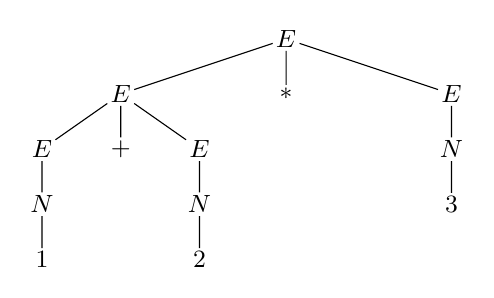
\begin{tikzpicture}[level distance=7mm,every node/.style={font=\small,inner sep=1pt},
   level 1/.style={sibling distance=21mm},level 2/.style={sibling distance=10mm},level 3/.style={sibling distance=7mm}]
\node{$E$}
  child {node{$E$}
    child {node{$E$} child{node{$N$} child{node{$1$}}}}
    child {node{$+$}}
    child {node{$E$} child{node{$N$} child{node{$2$}}}}
  }
  child {node{$*$}}
  child {node{$E$} child{node{$N$} child{node{$3$}}}};
\end{tikzpicture}
\hspace{1.2cm}
% Strom 2: 1+(2*3)
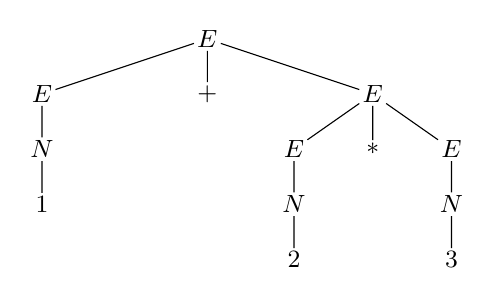
\begin{tikzpicture}[level distance=7mm,every node/.style={font=\small,inner sep=1pt},
   level 1/.style={sibling distance=21mm},level 2/.style={sibling distance=10mm},level 3/.style={sibling distance=7mm}]
\node{$E$}
  child {node{$E$} child{node{$N$} child{node{$1$}}}}
  child {node{$+$}}
  child {node{$E$}
    child {node{$E$} child{node{$N$} child{node{$2$}}}}
    child {node{$*$}}
    child {node{$E$} child{node{$N$} child{node{$3$}}}}
  };
\end{tikzpicture}
\end{center}
\obrpopis{dva derivační stromy slova \texttt{1+2*3} pro víceznačnou gramatiku $E\to E{+}E\mid E{*}E\mid N$, $N\to 1\mid 2\mid 3$. Vlevo strom čte výraz jako $(1{+}2){*}3$, vpravo jako $1{+}(2{*}3)$ -- dvě \emph{různá} ohodnocení téhož slova. Odstranění víceznačnosti (priorita, asociativita) vyžaduje pomocné neterminály, např.\ $E\to E{+}T\mid T$, $T\to T{*}N\mid N$.}

\subsection{Chomského normální forma}

Pro mnoho úvah (i pro rozhodování příslušnosti slova) se hodí gramatika s co nejjednoduššími pravidly.

\begin{definice}[Chomského normální forma]
CFG je v \emph{Chomského normální formě} (ChNF), obsahuje-li jen pravidla tvaru $A\to BC$ a $A\to a$ (kde $A,B,C\in V$, $a\in T$), případně $S\to\lambda$ -- a pak se $S$ nevyskytuje na pravé straně žádného pravidla.
\end{definice}

\begin{veta}[Převod do ChNF]
Ke každé bezkontextové gramatice existuje ekvivalentní gramatika v Chomského normální formě.
\end{veta}

\begin{intuice}
Převod je posloupnost úprav, z nichž každá odstraní jeden zakázaný typ pravidla a zachová jazyk: (1) odstíníme $S$ z pravých stran; (2) terminály v delších pravidlech nahradíme novými neterminály $T_a\to a$; (3) dlouhé pravé strany rozdělíme na dvojice novými neterminály; (4) odstraníme $\lambda$-pravidla (přes \emph{nulovatelné} neterminály, z nichž lze odvodit $\lambda$) a (5) jednotková pravidla $A\to B$ (přes jejich tranzitivní uzávěr).
\end{intuice}

\begin{poznamka}
ChNF dává rozhodovací algoritmus pro příslušnost slova: \textbf{CYK} (dynamické programování přes podslova) rozhodne $w\in L(G)$ v čase $O(n^3)$. Bezkontextové jazyky mají také \emph{iterační lemma} (rozklad $w=uvxyz$ s $|vxy|\le n$, $|vy|>0$ a $uv^kxy^kz\in L$), kterým se dokazuje, že např.\ $\{a^nb^nc^n\}$ \emph{není} bezkontextový. Třída je uzavřená na sjednocení, zřetězení, iteraci a otočení, \emph{ne} na průnik a doplněk.
\end{poznamka}

\subsection{Zásobníkový automat (PDA)}

\begin{definice}[Zásobníkový automat]
\emph{Zásobníkový automat} (PDA) je sedmice $P=(Q,\Sigma,\Gamma,\delta,q_0,Z_0,F)$, kde
\begin{itemize}
  \item $Q$ konečná množina stavů, $\Sigma$ vstupní abeceda, $\Gamma$ \emph{zásobníková abeceda},
  \item $\delta\colon Q\times(\Sigma\cup\{\lambda\})\times\Gamma\to\mathcal P_{\mathrm{FIN}}(Q\times\Gamma^*)$ přechodová funkce,
  \item $q_0\in Q$ počáteční stav, $Z_0\in\Gamma$ \emph{počáteční zásobníkový symbol}, $F\subseteq Q$ přijímající stavy.
\end{itemize}
Přechod $(q,\gamma)\in\delta(p,a,X)$ znamená: ve stavu $p$ přečti $a$ (nebo nečti nic, je-li $a=\lambda$), vrchol zásobníku $X$ \emph{nahraď} řetězcem $\gamma$ a přejdi do $q$. ($\Gamma^*$ jsou všechny konečné řetězce nad zásobníkovou abecedou, tj.\ možný nový vrchol; index $\mathrm{FIN}$ žádá \emph{konečnou} množinu přechodů z dané konfigurace.)
\end{definice}

\begin{definice}[Situace, krok, přijímaný jazyk]
\emph{Situace} (ID) je trojice $(q,w,\gamma)$: stav, zbývající vstup, obsah zásobníku (vrchol vlevo). Krok $\vdash$: je-li $(q,\alpha)\in\delta(p,a,X)$, pak $(p,aw,X\beta)\vdash(q,w,\alpha\beta)$; $\vdash^*$ je jeho uzávěr. Pro PDA definujeme \emph{dva} módy přijímání:
\[ L(P)=\{w\mid (q_0,w,Z_0)\vdash^*(q,\lambda,\alpha),\ q\in F\}\quad(\text{koncovým stavem}), \]
\[ N(P)=\{w\mid (q_0,w,Z_0)\vdash^*(q,\lambda,\lambda)\}\quad(\text{prázdným zásobníkem}). \]
Oba módy přijímají tutéž třídu (lze mezi nimi převádět); při přijímání prázdným zásobníkem je $F$ nepodstatné a vynechává se.
\end{definice}

\begin{intuice}
PDA je $\lambda$-NFA, ke kterému jsme přidali \emph{zásobník}: nedeterminismus „hádá`` (např.\ kde je střed slova), zásobník pamatuje neomezeně mnoho informace, ale jen z vrcholu (LIFO). Právě tato omezená paměť dělá z PDA přesný protějšek bezkontextových gramatik. \textbf{Deterministické} PDA jsou slabší -- přijímají jen vlastní podtřídu bezkontextových jazyků.
\end{intuice}

\begin{center}
\scalebox{1.2}{%
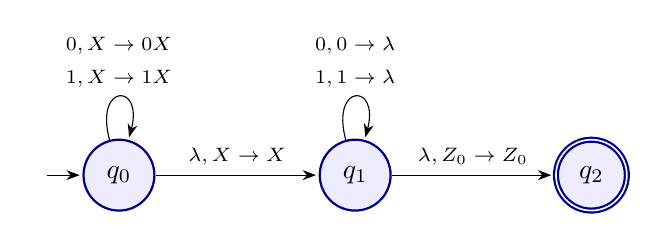
\begin{tikzpicture}[aut,node distance=3.0cm]
  \node[state,initial,initial text={}] (q0) {$q_0$};
  \node[state] (q1) [right=of q0] {$q_1$};
  \node[state,accepting] (q2) [right=of q1] {$q_2$};
  \path (q0) edge[loop above] node[align=center]{\scriptsize $0,X\to 0X$\\ \scriptsize $1,X\to 1X$} (q0)
        (q0) edge node{\scriptsize $\lambda,X\to X$} (q1)
        (q1) edge[loop above] node[align=center]{\scriptsize $0,0\to\lambda$\\ \scriptsize $1,1\to\lambda$} (q1)
        (q1) edge node{\scriptsize $\lambda,Z_0\to Z_0$} (q2);
\end{tikzpicture}%
}
\end{center}
\obrpopis{PDA přijímající $L_{ww^R}=\{ww^R\mid w\in\{0,1\}^*\}$ koncovým stavem. Hrana $a,X\to\alpha$ znamená $(q,\alpha)\in\delta(p,a,X)$; $X$ je libovolný vrchol ($X\in\{0,1,Z_0\}$). V $q_0$ automat \emph{ukládá} čtené znaky na zásobník; $\lambda$-přechodem do $q_1$ \emph{uhodne střed}; v $q_1$ \emph{odmazává} shodné znaky z vrcholu; vidí-li $Z_0$ (zásobník vyčerpán až na dno), $\lambda$-přechodem přijme. Nedeterminismus zajistí, že se uhodne správný střed pro každé $ww^R$.}

\begin{priklad}[SZZ podzim 2023 č.~2: Zásobníkový automat]
\szzotazka{podzim 2023}{2}{Zásobníkový automat (definice + konstrukce PDA)}\par
\textbf{Zadání.}\par
(1) Uveďte definici PDA. (2) Sestrojte PDA $A$ přijímající právě $w\in\{a,b\}^*$ s \emph{více $a$ než $b$} a zároveň \emph{lichým počtem $a$}: $L(A)=\{w\mid |w|_a>|w|_b\ \&\ |w|_a$ liché$\}$.

\smallskip
\textbf{Řešení.}\par
\textbf{(1)} Sedmice $(Q,\Sigma,\Gamma,\delta,q_0,Z_0,F)$ jako v definici výše.

\textbf{(2)} Na zásobníku udržujeme \emph{přebytek}: rozdíl $|w|_a-|w|_b$. Je-li kladný, leží na zásobníku tolik symbolů $A$ (nad $Z_0$); je-li záporný, tolik $B$. Čtené $a$ buď odmaže $B$ (přebytek $b$ klesá), nebo přidá $A$; čtené $b$ symetricky. \emph{Paritu} počtu $a$ držíme ve stavu: $q_0$ (sudě), $q_1$ (liše). Stavy $\{q_0,q_1,q_f\}$, $\Gamma=\{Z_0,A,B\}$, počátek $q_0$, $F=\{q_f\}$. Přechody (čtení $a$ překlápí $q_0\!\leftrightarrow\! q_1$):
\[
\begin{aligned}
&\delta(q_i,a,Z_0)=\{(q_{1-i},AZ_0)\},\ \delta(q_i,a,A)=\{(q_{1-i},AA)\},\ \delta(q_i,a,B)=\{(q_{1-i},\lambda)\},\\
&\delta(q_i,b,Z_0)=\{(q_i,BZ_0)\},\ \delta(q_i,b,B)=\{(q_i,BB)\},\ \delta(q_i,b,A)=\{(q_i,\lambda)\}\qquad(i\in\{0,1\}),\\
&\delta(q_1,\lambda,A)=\{(q_f,A)\}\quad(\text{přijmi: lichý počet $a$ a vrchol $A$, tj.\ přebytek $a$}).
\end{aligned}
\]
Přijímáme \emph{koncovým stavem}: do $q_f$ se dostaneme jen z $q_1$ (lichý počet $a$) a jen je-li na vrcholu $A$, což nastane právě když $|w|_a>|w|_b$. Správnost ověřena vyčerpáním slov do délky $11$ (Python). (Originál uvádí jinou (rovněž 3-stavovou) variantu, její diagram je v \texttt{priklady/}; za částečné řešení se uznával i automat jen pro „více $a$ než $b$``.)
\end{priklad}

\subsection{Ekvivalence CFG \texorpdfstring{$\leftrightarrow$}{<->} PDA a převody}

\begin{veta}[CFG $=$ PDA]
Jazyk je bezkontextový (generovaný CFG) právě tehdy, je-li přijímaný nějakým (nedeterministickým) zásobníkovým automatem.
\end{veta}

\begin{intuice}
Standardní směr CFG $\to$ PDA dá \emph{jednostavový} automat přijímající \emph{prázdným zásobníkem}, který na zásobníku simuluje \emph{levou derivaci} (v každém kroku se přepisuje nejlevější neterminál): zásobník drží dosud neodvozený zbytek věty. Pro $P=(\{q_0\},T,V\cup T,\delta,q_0,S)$:
\[ \delta(q_0,\lambda,A)=\{(q_0,\omega)\mid (A\to\omega)\in\mathcal P\}\ \text{(rozepiš neterminál)},\quad \delta(q_0,a,a)=\{(q_0,\lambda)\}\ \text{(odečti terminál)}. \]
Automat tak střídá „rozepsání neterminálu na vrcholu`` a „spárování terminálu se vstupem``; přijme prázdným zásobníkem právě slova generovaná $G$.
\end{intuice}

\begin{priklad}[SZZ léto 2023 č.~2: Převod gramatiky na automat]
\szzotazka{léto 2023}{2}{Převod bezkontextové gramatiky na automat (CFG $\to$ zásobníkový automat)}\par
\textbf{Zadání.}\par
(1) Definice CFG. (2) Sestrojte CFG $G$ pro $L=\{a^ib^j\mid i,j\ge 0,\ 2i=3j\}$. (3) Převeďte $G$ na PDA přijímající prázdným zásobníkem.

\smallskip
\textbf{Řešení.}\par
\textbf{(1)} Čtveřice $G=(V,T,\mathcal P,S)$ jako v definici výše.

\textbf{(2)} Z $2i=3j$ plyne $i=3k$, $j=2k$ pro $k\ge 0$, tj.\ $L=\{a^{3k}b^{2k}\mid k\ge 0\}$. Generuje ho
\[ G=(\{S\},\{a,b\},\{\,S\to aaa\,S\,bb\ \mid\ \lambda\,\},S). \]
(Ověřeno vyčerpáním do délky $12$: $L(G)$ se přesně shoduje s $\{a^ib^j:2i=3j\}$.)

\textbf{(3)} Jednostavový PDA $P=(\{q_0\},\{a,b\},\{a,b,S\},\delta,q_0,S)$ přijímající prázdným zásobníkem:
\[ \delta(q_0,\lambda,S)=\{(q_0,aaaSbb),\,(q_0,\lambda)\},\quad \delta(q_0,a,a)=\{(q_0,\lambda)\},\quad \delta(q_0,b,b)=\{(q_0,\lambda)\}. \]
První skupina rozepisuje $S$ podle pravidel, druhá páruje terminály se vstupem.\par
\emph{(V originálním PDF tato otázka nemá náčrt řešení; řešení je vlastní, ověřené numericky.)}
\end{priklad}

Stejnou „reprezentaci dvěma způsoby`` (gramatika \emph{i} automat) žádá i následující otázka.

\begin{priklad}[SZZ jaro 2024 č.~1: Reprezentace bezkontextového jazyka]
\szzotazka{jaro 2024}{1}{Reprezentace bezkontextového jazyka (CFG, zásobníkový automat)}\par
\textbf{Zadání.}\par
Pro $L=\{w\#s^R\mid w,s\in\{0,1\}^*,\ s$ je podslovo $w\}$ nad $\{0,1,\#\}$: (1) definice CFG a PDA, (2) CFG pro $L$, (3) PDA pro $L$.

\smallskip
\textbf{Řešení.}\par
\textbf{(1)} Definice CFG a PDA jsou výše.

\textbf{(2)} Slovo má tvar $w\#s^R$, kde $w=p\,u\,q$ a $s=u$ je souvislé podslovo. Necháme $A$ generovat libovolné slovo nad $\{0,1\}$ (prefix $p$ a suffix $q$), a párová pravidla $X$ budují $u$ vlevo i $u^R$ vpravo kolem $\#$:
\[ G=(\{S,X,A\},\{0,1,\#\},\mathcal P,S),\quad \mathcal P=\{\,S\to AX,\ X\to 0X0\mid 1X1\mid A\#,\ A\to 0A\mid 1A\mid\lambda\,\}. \]
($S\Rightarrow AX\Rightarrow p\,(u\,A\#\,u^R)$, tedy $w=p\,u\,q$ a za $\#$ stojí $u^R$.) Ověřeno vyčerpáním do délky~$9$.

\textbf{(3)} Standardním převodem $G$ na jednostavový PDA $(\{q_0\},\{0,1,\#\},\{0,1,\#,S,X,A\},\delta,q_0,S)$ přijímající prázdným zásobníkem, kde přechody odpovídají pravidlům a~čtení písmen:
\[ \delta=\{((q_0,\lambda,H),\beta)\mid H\to\beta\in\mathcal P\}\cup\{((q_0,a,a),\lambda)\mid a\in\{0,1,\#\}\}. \]
(Alternativně přímo: čteme $w$ a~ukládáme znaky na zásobník; po $\#$ nejprve $\lambda$-přechody smažeme libovolný počet symbolů (odhad konce $u$), pak párujeme $s^R$ se zásobníkem a~nakonec ho vyprázdníme.)
\end{priklad}

Poslední otázka kombinuje bezkontextový a regulární jazyk. \emph{Průnik} bezkontextového a regulárního jazyka je opět bezkontextový -- získáme ho \emph{součinem} PDA a DFA (stavy nesou dvojici, zásobník zůstává jeden).

\begin{priklad}[SZZ jaro 2025 č.~1: Průnik bezkontextového a regulárního jazyka]
\szzotazka{jaro 2025}{1}{Průnik bezkontextového a regulárního jazyka (PDA, CFG $\cap$ DFA)}\par
\textbf{Zadání.}\par
$L_1=L(G)$ pro $G=(\{S\},\{0,1\},\{S\to SS\mid 0S1\mid\lambda\},S)$ (vyvážené závorky: $0$ otevírá, $1$ zavírá), $L_2=L(A)$ pro daný DFA $A$ se stavy $\{q_0,q_1,q_2,q_3\}$, který přijímá ve \emph{všech} stavech ($F=\{q_0,q_1,q_2,q_3\}$) a má přechody $\delta_A(q_0,1)=q_0$, $\delta_A(q_0,0)=q_1$, $\delta_A(q_1,0)=q_1$, $\delta_A(q_1,1)=q_2$, $\delta_A(q_2,0)=q_3$, $\delta_A(q_2,1)=q_0$, $\delta_A(q_3,0)=q_1$; přechod $\delta_A(q_3,1)$ \emph{chybí}. Sestrojte PDA pro $L=L_1\cap L_2$.

\smallskip
\textbf{Řešení.}\par
Použijeme \emph{součinovou konstrukci}: přijímání DFA $A$ simulujeme \emph{stavem}, generování $G$ \emph{zásobníkem} (jako u převodu CFG na jednostavový PDA). Výsledný PDA $P=(\{q_0,q_1,q_2,q_3\},\{0,1\},\{0,1,S\},\delta_P,q_0,S)$ přijímá prázdným zásobníkem:
\[
\begin{aligned}
\delta_P(q_i,a,a)&=\{(\delta_A(q_i,a),\lambda)\}\quad a\in\{0,1\}\ \text{(čti terminál, posuň DFA)},\\
\delta_P(q_i,\lambda,S)&=\{(q_i,SS),(q_i,0S1),(q_i,\lambda)\}\quad\text{(krok derivace $G$, stav DFA beze změny)}.
\end{aligned}
\]
PDA vyprázdní zásobník právě tehdy, když $S\Rightarrow^* w$, tj.\ $w\in L_1$; jeho stavová složka přitom sleduje $\delta_A^*(q_0,w)$. Tato součinová konstrukce dokazuje, že \emph{průnik bezkontextového a~regulárního jazyka je bezkontextový}. Je \emph{generická} v~$\delta_A$: konkrétní přechody DFA do ní vstupují jen symbolicky.

\emph{Proč stačí přijímat prázdným zásobníkem.} Stav $q_3$ znamená „slovo zatím končí na $010$`` a~chybí mu přechod na $1$, takže $A$ na slově s~podslovem $0101$ uvízne. Protože jsou všechny stavy přijímající, je $L_2=\{w\mid w$ neobsahuje $0101\}$ (ne celé $\{0,1\}^*$) a~$L$ tvoří vyvážená slova bez podslova $0101$; např.\ $0011\in L$, ale $0101\in L_1\setminus L_2$. Chybějící přechod DFA se v~$P$ projeví tak, že $P$ nemůže přečíst další znak a~výpočet skončí neúspěchem; jinak je každý dosažený stav DFA přijímající, takže kontrola koncového stavu není potřeba. (Obecně, kdyby $F_A\neq Q_A$, vložíme pod $S$ nové dno $Z_0$ a~přidáme přechody $\delta_P(q,\lambda,Z_0)=\{(q,\lambda)\}$ jen pro $q\in F_A$.) Správnost ověřena vyčerpáním slov do délky~$12$ (Python).\par
\emph{Stavový diagram DFA $A$ je v} \texttt{priklady/}.
\end{priklad}

% ============================================================
\section{Rekurzivně spočetné jazyky (Turingův stroj, nerozhodnutelnost)}

Nejširší třída Chomského hierarchie odpovídá \emph{nejobecnějšímu} modelu výpočtu -- Turingovu stroji -- a \emph{nejobecnějším} gramatikám (typ~0). Zde už narazíme na hranici algoritmické řešitelnosti: existují přesně definované problémy, které \emph{žádný} algoritmus nerozhodne.

\subsection{Turingův stroj}

\begin{definice}[Turingův stroj]
\emph{Turingův stroj} (TM) je sedmice $M=(Q,\Sigma,\Gamma,\delta,q_0,\sqcup,F)$, kde
\begin{itemize}
  \item $Q$ konečná množina stavů, $q_0\in Q$ počáteční, $F\subseteq Q$ přijímající stavy,
  \item $\Sigma$ vstupní abeceda, $\Gamma\supsetneq\Sigma$ \emph{pásková abeceda}, $\sqcup\in\Gamma\setminus\Sigma$ \emph{prázdný symbol} (mezera),
  \item $\delta\colon (Q\setminus F)\times\Gamma\to Q\times\Gamma\times\{\leftarrow,\to\}$ přechodová funkce (může být parciální).
\end{itemize}
Stroj má oboustranně nekonečnou \emph{pásku}; v každém kroku přečte znak pod hlavou, podle $\delta$ jej přepíše, změní stav a posune hlavu doleva/doprava. \emph{Konfigurace} popisuje stav, obsah pásky a polohu hlavy.
\end{definice}

\begin{center}
\scalebox{1.2}{%
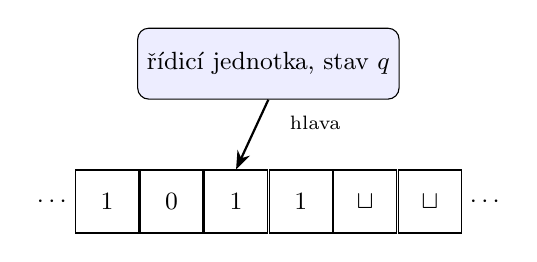
\begin{tikzpicture}[>=Stealth,
   cell/.style={draw,minimum size=8mm,font=\small},
   ctrl/.style={draw,rounded corners,fill=blue!7,minimum width=30mm,minimum height=9mm,font=\small}]
  \foreach \i/\s in {0/{$1$},1/{$0$},2/{$1$},3/{$1$},4/{$\sqcup$},5/{$\sqcup$}} \node[cell] (c\i) at (\i*0.82,0) {\s};
  \node[font=\small] at (-0.7,0) {$\cdots$};
  \node[font=\small] at (5*0.82+0.7,0) {$\cdots$};
  \node[ctrl] (ctrl) at (2.05,1.75) {řídicí jednotka, stav $q$};
  \draw[->,thick] (ctrl.south) -- (c2.north);
  \node[font=\scriptsize,right] at (2.2,1.0) {hlava};
\end{tikzpicture}%
}
\end{center}
\obrpopis{Turingův stroj. Konečná \emph{řídicí jednotka} (v jednom z konečně mnoha stavů) ovládá \emph{hlavu} pohybující se po oboustranně nekonečné pásce. Na rozdíl od konečného automatu smí znak pod hlavou \emph{přepsat} a pohybovat se \emph{oběma směry} -- to dává neomezenou pracovní paměť. Na počátku je na pásce vstup, jinde mezery $\sqcup$; hlava stojí na prvním znaku, jednotka ve stavu $q_0$.}

\begin{definice}[Přijímaný a rozhodovaný jazyk; R a RE]
Stroj $M$ \emph{přijme} slovo $w$, dojde-li jeho výpočet do přijímajícího stavu (jinak slovo odmítne, nebo se nezastaví). \emph{Jazyk přijímaný} $M$ je $L(M)=\{w\mid M$ přijme $w\}$.
\begin{itemize}
  \item Jazyk je \emph{rekurzivně spočetný} (částečně rozhodnutelný), třída $\mathrm{RE}$, je-li $L=L(M)$ pro nějaký TM (na slovech mimo $L$ se stroj smí \emph{zacyklit}).
  \item Jazyk je \emph{rozhodnutelný} (rekurzivní), třída $\mathrm R$, existuje-li TM, který se na \emph{každém} vstupu zastaví a přijímá $L$.
\end{itemize}
\end{definice}

\begin{intuice}
Rozdíl R vs.\ RE je v garanci zastavení. \emph{Rozhodující} stroj vždy odpoví ano/ne. \emph{Přijímající} stroj řekne „ano`` na slovech jazyka, ale na slovech mimo jazyk se může točit donekonečna -- nikdy se nedozvíme „ne``. Platí $\mathrm R\subseteq\mathrm{RE}$ (rozhodující stroj je speciálním případem přijímajícího); uvidíme, že inkluze je \emph{ostrá}.
\end{intuice}

\subsection{Gramatiky typu 0}

\begin{definice}[Gramatika typu 0]
\emph{Gramatika typu 0} (obecná) má pravidla $\alpha\to\beta$, kde $\alpha,\beta\in(V\cup T)^*$ a $\alpha$ obsahuje aspoň jeden neterminál (levá strana smí být libovolné slovo, ne jen jediný neterminál jako u CFG).
\end{definice}

\begin{veta}[Typ 0 $=$ RE]
Třída jazyků generovaných gramatikami typu 0 je přesně třída rekurzivně spočetných jazyků: $\mathcal L_0=\mathrm{RE}$.
\end{veta}

\begin{intuice}
Gramatika typu 0 a Turingův stroj jsou dvě strany téže mince. Gramatikou lze \emph{simulovat výpočet} stroje (pravidla přepisují konfiguraci na následující), a naopak stroj umí \emph{vyjmenovávat} všechna slova odvoditelná gramatikou a porovnávat je se vstupem. Proto „generovatelné gramatikou`` $=$ „přijímané strojem`` $=$ rekurzivně spočetné.
\end{intuice}

\subsection{Algoritmicky nerozhodnutelné problémy}

Že některé jazyky nejsou rozhodnutelné (ba ani rekurzivně spočetné), plyne z \emph{diagonálního} argumentu. Turingovy stroje (nad $\{0,1\}$) lze \emph{zakódovat} do slov; slovo $\alpha$ kóduje stroj $M_\alpha$.

\begin{definice}[Univerzální a diagonální jazyk]
\emph{Univerzální jazyk} $L_u=\{\langle\alpha,\beta\rangle\mid \beta\in L(M_\alpha)\}$ obsahuje dvojice „kód stroje, vstup``, kde stroj vstup přijme. \emph{Diagonální jazyk} $L_d=\{\alpha\mid \alpha\notin L(M_\alpha)\}$ obsahuje kódy strojů, které \emph{nepřijmou samy sebe}.
\end{definice}

\begin{veta}[Nerozhodnutelnost]
$L_u$ je rekurzivně spočetný, ale \emph{není} rozhodnutelný. $L_d$ není ani rekurzivně spočetný. Inkluze $\mathrm R\subsetneq\mathrm{RE}$ je tedy ostrá.
\end{veta}

\begin{proof}[Důkaz \textnormal{(nepovinný -- diagonalizace)}]
$L_u$ přijímá \emph{univerzální stroj} (UTM), který odsimuluje $M_\alpha$ na $\beta$ -- proto $L_u\in\mathrm{RE}$. Kdyby byl $L_d$ rekurzivně spočetný, přijímal by ho nějaký $M_\gamma$, tedy $L_d=L(M_\gamma)$. Pak ale
\[ \gamma\in L_d \iff \gamma\notin L(M_\gamma) \iff \gamma\notin L_d, \]
spor. Takže $L_d\notin\mathrm{RE}$. Odtud $L_u\notin\mathrm R$: platí $\alpha\in L_d\iff\langle\alpha,\alpha\rangle\notin L_u$, takže kdyby byl $L_u$ rozhodnutelný, rozhodli bychom i $L_d$ (spustit rozhodovací stroj pro $L_u$ na $\langle\alpha,\alpha\rangle$ a odpověď obrátit) -- spor.
\end{proof}

\begin{poznamka}[Problém zastavení a Postova věta]
Týž argument dává \emph{problém zastavení} (halting problem): neexistuje algoritmus, který pro libovolný program a vstup rozhodne, zda se výpočet zastaví. Užitečné kritérium dává \emph{Postova věta}: jazyk $L$ je rozhodnutelný \emph{právě tehdy}, když $L$ i jeho doplněk $\overline L$ jsou rekurzivně spočetné. (Proto $L_u$, jehož doplněk není RE, rozhodnutelný být nemůže.)
\end{poznamka}

% ============================================================
\section{Chomského hierarchie a zařazování jazyků}

Předchozí tři sekce probraly tři ze čtyř pater \emph{Chomského hierarchie}. Teď je uspořádáme do jednoho obrázku a doplníme chybějící patro -- \emph{kontextové} (typ~1) jazyky -- a ukážeme, jak \emph{zařadit konkrétní jazyk}.

\subsection{Klasifikace gramatik a hierarchie}

\begin{definice}[Chomského hierarchie]
Gramatiky (a jimi generované třídy jazyků) klasifikujeme podle tvaru pravidel:
\begin{itemize}
  \item \textbf{typ 0} (rekurzivně spočetné $\mathcal L_0$): $\alpha\to\beta$, $\alpha$ obsahuje neterminál;
  \item \textbf{typ 1} (kontextové $\mathcal L_1$): $\gamma A\beta\to\gamma\omega\beta$ s $\omega\neq\lambda$ (přepis $A$ \emph{v kontextu} $\gamma,\beta$; výjimkou je $S\to\lambda$, pak se $S$ nevyskytuje vpravo). Ekvivalentně \emph{monotónní} (nezkracující) pravidla $|\alpha|\le|\beta|$;
  \item \textbf{typ 2} (bezkontextové $\mathcal L_2$): $A\to\omega$;
  \item \textbf{typ 3} (regulární $\mathcal L_3$): $A\to wB$, $A\to w$.
\end{itemize}
\end{definice}

\begin{veta}[Uspořádání hierarchie]
Třídy tvoří ostrou hierarchii
\[ \mathcal L_3\subsetneq\mathcal L_2\subsetneq\mathcal L_1\subsetneq\mathcal L_0, \]
a navíc $\mathcal L_2\subsetneq\mathrm R$, $\mathcal L_1\subsetneq\mathrm R\subsetneq\mathrm{RE}=\mathcal L_0$. Každému patru odpovídá typ automatu.
\end{veta}

\begin{center}
\scalebox{1.2}{%
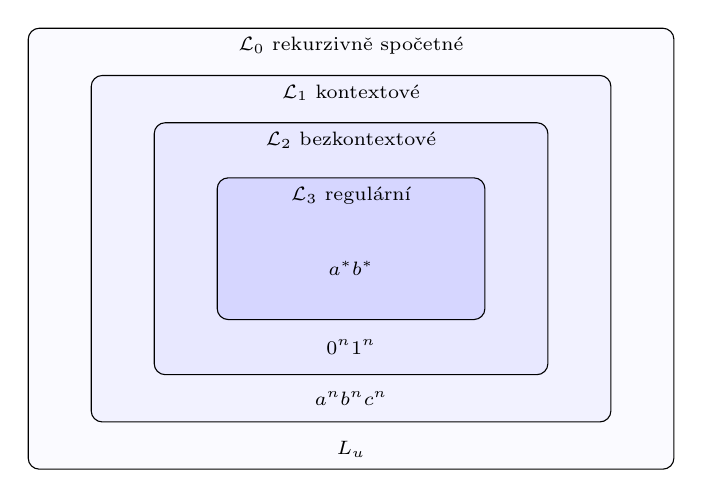
\begin{tikzpicture}[font=\small,
   lev/.style={draw,rounded corners,inner sep=0pt}]
  \node[lev,minimum width=82mm,minimum height=56mm,fill=blue!2] (l0) at (0,0) {};
  \node[lev,minimum width=66mm,minimum height=44mm,fill=blue!5] (l1) at (0,0) {};
  \node[lev,minimum width=50mm,minimum height=32mm,fill=blue!9] (l2) at (0,0) {};
  \node[lev,minimum width=34mm,minimum height=18mm,fill=blue!16] (l3) at (0,0) {};
  \node[font=\scriptsize,anchor=north] at (l0.north) {$\mathcal L_0$ rekurzivně spočetné};
  \node[font=\scriptsize,anchor=north] at (l1.north) {$\mathcal L_1$ kontextové};
  \node[font=\scriptsize,anchor=north] at (l2.north) {$\mathcal L_2$ bezkontextové};
  \node[font=\scriptsize,anchor=north] at (l3.north) {$\mathcal L_3$ regulární};
  \node[font=\scriptsize] at (0,-0.25) {$a^*b^*$};
  \node[font=\scriptsize] at (0,-1.25) {$0^n1^n$};
  \node[font=\scriptsize] at (0,-1.9) {$a^nb^nc^n$};
  \node[font=\scriptsize] at (0,-2.55) {$L_u$};
\end{tikzpicture}%
}
\end{center}
\obrpopis{Chomského hierarchie. Každá třída je vlastní podmnožinou třídy o~patro výš (vnořené obdélníky). Příklady svědčící o ostrosti: $0^n1^n$ je bezkontextový, ne regulární; $a^nb^nc^n$ je kontextový, ne bezkontextový; univerzální jazyk $L_u$ je rekurzivně spočetný, ne rozhodnutelný (a $\mathrm R$ leží mezi $\mathcal L_1$ a $\mathcal L_0$). Soulad automatů, gramatik a jazyků shrnuje tabulka níže.}

\begin{center}\small
\begin{tabular}{llll}
\toprule
typ & gramatika & automat & uzávěr na operace\\
\midrule
3 & pravá lineární & konečný automat (DFA/NFA) & vše ($\cup,\cap,\overline{\phantom{x}},\cdot,{}^*,{}^R$)\\
2 & bezkontextová & zásobníkový automat (PDA) & $\cup,\cdot,{}^*,{}^R$ (ne $\cap$, ne $\overline{\phantom{x}}$)\\
1 & kontextová (monotónní) & lineárně omezený automat (LBA) & vše\\
0 & obecná (typ 0) & Turingův stroj & $\cup,\cap,\cdot,{}^*,{}^R$ (ne $\overline{\phantom{x}}$)\\
\bottomrule
\end{tabular}
\end{center}
{\small Lineárně omezený automat (LBA) je Turingův stroj, který smí použít jen pásku délky vstupu (ohraničenou zarážkami).}

\subsection{Zařazení konkrétního jazyka}

Požadavky okruhu zahrnují \emph{zařazení konkrétního jazyka do hierarchie} se zdůvodněním. Postup má dvě strany:

\begin{intuice}
\textbf{Horní zařazení (do třídy patří):} sestroj automat nebo gramatiku příslušného typu -- tím dokážeš, že jazyk \emph{do třídy patří}. \textbf{Dolní mez (do nižší třídy nepatří):} použij \emph{iterační lemma} (regulární resp.\ bezkontextové) a najdi slovo, které napumpováním vypadne z jazyka -- tím dokážeš, že jazyk do nižší třídy \emph{nepatří}.
\end{intuice}

\begin{priklad}[Zařazení tří typických jazyků]
\textbf{Zadání.} Zařaďte do Chomského hierarchie: (a) $\{a^nb^n\mid n\ge 0\}$, (b) $\{a^nb^nc^n\mid n\ge 0\}$, (c) $\{ww\mid w\in\{0,1\}^*\}$.

\smallskip
\textbf{Řešení.}\par
\textbf{(a)} \emph{Bezkontextový, ne regulární} ($\mathcal L_2\setminus\mathcal L_3$). Gramatika $S\to aSb\mid\lambda$ jej generuje (horní zařazení). Neregularitu dá iterační lemma: pro $w=a^nb^n$ leží napumpovaná část $y$ v úvodních $a$, takže $a^{n+|y|}b^n\notin L$.

\textbf{(b)} \emph{Kontextový, ne bezkontextový} ($\mathcal L_1\setminus\mathcal L_2$). Bezkontextové iterační lemma na $a^nb^nc^n$ ukáže, že napumpování rozbije rovnost počtů (úsek $vxy$ délky $\le n$ nemůže obsahovat všechna tři písmena). Patří ale do $\mathcal L_1$, generuje ho monotónní gramatika
\[ S_0\to S\mid\lambda,\quad S\to aSBC\mid aBC,\quad CB\to BC,\quad aB\to ab,\quad bB\to bb,\quad bC\to bc,\quad cC\to cc \]
(pravidlo $CB\to BC$ přesune všechna $B$ před $C$, zbylá pravidla je pak zleva doprava přepíšou na terminály; ověřeno vyčerpáním do délky~$12$).

\textbf{(c)} \emph{Kontextový, ne bezkontextový} ($\mathcal L_1\setminus\mathcal L_2$). „Kopírovací`` jazyk $\{ww\}$ rovněž odmítne bezkontextové iterační lemma (slovo $0^n1^n0^n1^n$). Do $\mathcal L_1$ patří, protože ho rozhodne lineárně omezený automat: ověří sudou délku, označováním znaků z~obou konců najde střed a obě poloviny porovná znak po znaku, vše jen v~prostoru vstupu. (Pozor: $\{ww^R\}$ -- palindromy sudé délky -- naopak \emph{bezkontextový} je (viz zásobníkový automat výše); rozdíl je v pořadí druhé kopie.)
\end{priklad}

% ============================================================
\section*{Shrnutí}
\addcontentsline{toc}{section}{Shrnutí}

\begin{poznamka}
\textbf{Klíčové vlastnosti a vzorce (přehled k~SZZ).} Stručný výčet klíčových definic, vět a vzorců okruhu I1. Zkratky: DFA $=$ deterministický, NFA $=$ nedeterministický konečný automat, CFG $=$ bezkontextová gramatika, PDA $=$ zásobníkový automat, TM $=$ Turingův stroj, CFL $=$ bezkontextový jazyk.

\smallskip
\emph{Regulární jazyky -- modely a~ekvivalence.}
\begin{itemize}
  \item \textbf{DFA} $(Q,\Sigma,\delta,q_0,F)$: $\delta\colon Q\times\Sigma\to Q$ totální (nebo parciální s~implicitním mrtvým stavem); rozšíření $\delta^*\colon Q\times\Sigma^*\to Q$ indukcí -- $\delta^*(q,\lambda)=q$, $\delta^*(q,wx)=\delta(\delta^*(q,w),x)$; jazyk $L(A)=\{w\mid\delta^*(q_0,w)\in F\}$.
  \item \textbf{NFA} $(Q,\Sigma,\delta,Q_0,F)$: $Q_0\subseteq Q$ množina počátečních stavů, $\delta\colon Q\times\Sigma\to 2^Q$; přijme, \emph{existuje-li} výpočet do~přijímajícího stavu. ($\lambda$-NFA navíc dovoluje přechody na $\lambda$; ekvivalentní NFA.)
  \item \textbf{Ekvivalence čtyř modelů:} DFA $=$ NFA ($\lambda$-NFA) $=$ regulární výrazy $=$ pravé lineární gramatiky (typ~3); vše popisuje třídu $\mathcal L_3$.
  \item \textbf{Regulární výraz} nad $\Sigma$: základ $\emptyset$, $\lambda$, $a\in\Sigma$; operace $+$ (sjednocení), $\cdot$ (zřetězení), ${}^*$ (iterace); značení $R^+\equiv RR^*$.
  \item \textbf{Pravá lineární gramatika} (typ~3): pravidla tvaru $A\to wB$ nebo $A\to w$; neterminál $=$ stav (přechod $A\xrightarrow{a}B$ odpovídá pravidlu $A\to aB$).
\end{itemize}

\smallskip
\emph{Klíčové převody u~regulárních jazyků.}
\begin{itemize}
  \item \textbf{Podmnožinová konstrukce} (NFA $\to$ DFA): stavy DFA jsou podmnožiny stavů NFA; $\delta_D(S,a)=\bigcup_{q\in S}\delta_N(q,a)$; počáteční stav $Q_0$ (množina počátečních stavů NFA); přijímající stavy -- podmnožiny obsahující stav NFA z~$F$. Může exponenciálně nafouknout stavový prostor ($2^n$ stavů v~nejhorším případě).
  \item \textbf{Kleeneho věta}: $L$ je regulární $\iff$ $L$ je popsatelný regulárním výrazem; výraz $\to$ $\lambda$-NFA Kleeneho stavebnicí (indukcí podle výrazu), automat $\to$ výraz eliminací stavů.
  \item \textbf{Doplněk} $\overline L$: totalizuj DFA (přidej mrtvý stav pro chybějící přechody), zaměň přijímající a~nepřijímající stavy; výsledek přijímá právě $\overline L$. (Jen pro DFA -- NFA neumí doplněk přímým záměněním stavů.)
  \item \textbf{Součin DFA} (průnik): pro $L_1\cap L_2$ sestav DFA se stavy $Q_1\times Q_2$, $\delta\bigl((p,q),a\bigr)=\bigl(\delta_1(p,a),\delta_2(q,a)\bigr)$, přijímající stavy $F_1\times F_2$.
\end{itemize}

\smallskip
\emph{Iterační lemma pro regulární jazyky (důkaz neregularity).}
\begin{itemize}
  \item Pro každý regulární jazyk $L$ existuje $n\ge 1$: každé $w\in L$ s~$|w|\ge n$ lze rozložit $w=xyz$ tak, že $y\neq\lambda$, $|xy|\le n$, a~$\forall k\ge 0\colon xy^kz\in L$.
  \item \textbf{Použití (dolní mez):} zvolíme $w\in L$ s~$|w|\ge n$, ukážeme, že pro \emph{každé} rozložení $xyz$ ($y\neq\lambda$, $|xy|\le n$) existuje $k$ takové, že $xy^kz\notin L$ -- spor s~lemmatem.
  \item Typické slovo: $a^nb^n$ (část $y$ leží v~úvodních $a$, napumpování poruší rovnost počtů).
\end{itemize}

\smallskip
\emph{Uzávěrové vlastnosti regulárních jazyků.}
\begin{itemize}
  \item Uzavřeno na: $\cup$, $\cap$, $\overline{\phantom{x}}$ (doplněk), $\cdot$ (zřetězení), ${}^*$, ${}^R$ (otočení).
\end{itemize}

\smallskip
\emph{Bezkontextové jazyky -- CFG a~normální formy.}
\begin{itemize}
  \item \textbf{CFG} $(V,T,\mathcal P,S)$: $V$ neterminály, $T$ terminály, $S\in V$ startovní symbol, $\mathcal P$ pravidla $A\to\omega$ ($A\in V$, $\omega\in(V\cup T)^*$). Jazyk $L(G)=\{w\in T^*\mid S\Rightarrow^* w\}$.
  \item Derivace $\Rightarrow$, $\Rightarrow^*$; \textbf{derivační strom} (parse tree); \textbf{víceznačnost} -- slovo má $\ge 2$ různé derivační stromy; nejednoznačný jazyk -- každá CFG jej generuje víceznačně.
  \item \textbf{Chomského normální forma (ChNF):} pravidla jen $A\to BC$ nebo $A\to a$ (povolena $S\to\lambda$ je-li $\lambda\in L$); každá CFG lze převést do ChNF.
  \item \textbf{CYK} (Cocke--Younger--Kasami): dynamické programování na trojúhelnické tabulce; $O(n^3)$; rozhoduje $w\in L(G)$ pro CFG v~ChNF.
\end{itemize}

\smallskip
\emph{Zásobníkový automat (PDA) -- definice a~módy přijímání.}
\begin{itemize}
  \item \textbf{PDA} je sedmice $(Q,\Sigma,\Gamma,\delta,q_0,Z_0,F)$: $\Gamma$ zásobníková abeceda, $Z_0\in\Gamma$ počáteční zásobníkový symbol, $\delta\colon Q\times(\Sigma\cup\{\lambda\})\times\Gamma\to\mathcal P_{\mathrm{FIN}}(Q\times\Gamma^*)$.
  \item \textbf{Situace} $(q,w,\gamma)$: aktuální stav, nezpracovaný vstup, obsah zásobníku (vrchol vlevo).
  \item \textbf{Přijímání koncovým stavem} $L(P)=\{w\mid(q_0,w,Z_0)\vdash^*(q_f,\lambda,\gamma),\ q_f\in F\}$; \textbf{prázdným zásobníkem} $N(P)=\{w\mid(q_0,w,Z_0)\vdash^*(q,\lambda,\lambda)\}$. Obě třídy jsou stejné: $L(P)=N(P')$ pro vhodné $P'$ a~naopak.
  \item PDA je obecně nedeterministický; deterministické PDA (DPDA) přijímají striktní podtřídu CFL.
\end{itemize}

\smallskip
\emph{Ekvivalence CFG a~PDA; průnik s~regulárním jazykem.}
\begin{itemize}
  \item \textbf{CFG $=$ PDA:} ke každé CFG existuje ekvivalentní PDA a~naopak; třída CFL $=$ třída jazyků přijímaných PDA.
  \item \textbf{CFG $\to$ jednostavový PDA} (přijímání prázdným zásobníkem): jeden stav $q_0$; pro každé pravidlo $A\to\alpha$: $\delta(q_0,\lambda,A)\ni(q_0,\alpha)$; pro každý terminál $a$: $\delta(q_0,a,a)\ni(q_0,\lambda)$. Simuluje levou derivaci.
  \item \textbf{Průnik CFL $\cap$ REG $\subseteq$ CFL:} součin PDA $\times$ DFA -- stavy $Q_P\times Q_D$, čtení symbolu posunuje oba automaty souběžně; zásobník zůstává zásobníkem PDA. Konstruktivní důkaz a~základ SZZ otázky jaro~2025.
\end{itemize}

\smallskip
\emph{Iterační lemma pro bezkontextové jazyky (důkaz, že jazyk není CFL).}
\begin{itemize}
  \item Pro každý CFL $L$ existuje $n\ge 1$: každé $w\in L$ s~$|w|\ge n$ lze rozložit $w=uvxyz$ tak, že $vy\neq\lambda$, $|vxy|\le n$, a~$\forall k\ge 0\colon uv^kxy^kz\in L$.
  \item \textbf{Použití:} pumping na $a^nb^nc^n$ -- $|vxy|\le n$ neumožňuje zahrnout všechna tři písmena; napumpování poruší rovnost počtů.
  \item Pozor: $\{ww^R\}$ (palindromy sudé délky) je bezkontextový -- PDA uloží první polovinu na zásobník, střed nedeterministicky uhodne a druhou polovinu porovná se zásobníkem.
\end{itemize}

\smallskip
\emph{Uzávěrové vlastnosti bezkontextových jazyků.}
\begin{itemize}
  \item Uzavřeno na: $\cup$, $\cdot$, ${}^*$, ${}^R$; průnik s~regulárním (viz výše).
  \item \textbf{Není} uzavřeno na: $\cap$ (průnik dvou CFL nemusí být CFL -- protipříkladem je $\{a^nb^nc^n\}=\{a^nb^nc^m\}\cap\{a^mb^nc^n\}$, průnik dvou CFL, který podle iteračního lemmatu CFL není), $\overline{\phantom{x}}$ (doplněk).
\end{itemize}

\smallskip
\emph{Rekurzivně spočetné jazyky a~Turingův stroj.}
\begin{itemize}
  \item \textbf{TM} sedmice $(Q,\Sigma,\Gamma,\delta,q_0,\sqcup,F)$: $\Sigma\subset\Gamma$ vstupní abeceda, $\sqcup\in\Gamma\setminus\Sigma$ blank; $\delta\colon (Q\setminus F)\times\Gamma\to Q\times\Gamma\times\{\leftarrow,\to\}$ (parciální).
  \item \textbf{R} (rekurzivní $=$ rozhodnutelné): TM se vždy zastaví (přijme, nebo se zastaví mimo $F$, tj.\ odmítne). \textbf{RE} (rekurzivně spočetné): TM přijme nebo cyklí. $\mathrm R\subsetneq\mathrm{RE}$.
  \item Gramatika \textbf{typu~0} (neomezená) $=$ RE: každý RE jazyk je generovatelný gramatikou bez omezení tvaru pravidel a~naopak.
\end{itemize}

\smallskip
\emph{Nerozhodnutelnost.}
\begin{itemize}
  \item \textbf{Diagonální jazyk} $L_d=\{\gamma_i\mid\gamma_i\notin L(M_i)\}\notin\mathrm{RE}$; důkaz diagonalizací.
  \item \textbf{Univerzální jazyk} $L_u=\{\langle M,w\rangle\mid M\text{ přijme }w\}\in\mathrm{RE}\setminus\mathrm R$; univerzální TM simuluje $M$ na $w$ -- přijme, ale nemůže vždy odmítnout.
  \item \textbf{Problém zastavení} (halting): neexistuje algoritmus rozhodující pro libovolný program a~vstup, zda výpočet skončí; nerozhodnutelnost plyne z~nerozhodnutelnosti $L_u$.
  \item \textbf{Postova věta}: $L\in\mathrm R\iff L\in\mathrm{RE}$ a~$\overline L\in\mathrm{RE}$. (Tedy $L_u$ není rozhodnutelný, protože $\overline{L_u}\notin\mathrm{RE}$.)
\end{itemize}

\smallskip
\emph{Chomského hierarchie -- přehled.}
\begin{itemize}
  \item Ostrá hierarchie: $\mathcal L_3\subsetneq\mathcal L_2\subsetneq\mathcal L_1\subsetneq\mathcal L_0$; odpovídající automaty: FA $\subsetneq$ PDA $\subsetneq$ LBA $\subsetneq$ TM.
  \item Tabulka souladu: typ~3 (pravá lin.\ gram., FA, uzavřeno na vše), typ~2 (CFG, PDA, uzavřeno na $\cup\cdot{}^*{}^R$, ne $\cap\overline{\phantom{x}}$), typ~1 (kontextová, LBA, uzavřeno na vše), typ~0 (obecná, TM, uzavřeno na $\cup\cap\cdot{}^*{}^R$, ne $\overline{\phantom{x}}$).
  \item \textbf{Vzorové jazyky:} $a^*b^*\in\mathcal L_3$; $\{a^nb^n\}\in\mathcal L_2\setminus\mathcal L_3$; $\{ww^R\}\in\mathcal L_2$ (PDA: push první polovina, pop druhá); $\{a^nb^nc^n\},\{ww\}\in\mathcal L_1\setminus\mathcal L_2$; $L_u\in\mathrm{RE}\setminus\mathrm R$; $L_d\notin\mathrm{RE}$.
  \item \textbf{Zařazení jazyka:} horní mez -- sestrojit automat nebo gramatiku příslušného typu; dolní mez -- aplikovat iterační lemma (regulární resp.\ bezkontextové) a~najít slovo, které napumpováním vypadne z~jazyka.
\end{itemize}
\end{poznamka}

\section*{Zdroje}
\addcontentsline{toc}{section}{Zdroje}

{\raggedright
\begin{itemize}
  \item M.~Vomlelová: \emph{Automaty a gramatiky}, slidy k~přednášce NTIN071, MFF UK, verze 2021 (primární zdroj rozsahu a~značení: DFA/NFA, regulární výrazy, gramatiky, zásobníkový automat, Turingův stroj, nerozhodnutelnost, Chomského hierarchie). Stránka přednášející a~kopie slidů ve státnicových materiálech T.~Slámy:\\ \url{https://ktiml.mff.cuni.cz/~marta/}\\ \url{https://slama.dev/assets/priprava-na-statnice-mff-uk/autogramy/slidy.pdf}
  \item M.~Mareš: \emph{Úvod do automatů}, studijní text, MFF UK (souvislý výklad regulárních a~bezkontextových jazyků, Turingových strojů a~nerozhodnutelnosti).\\ \url{https://mj.ucw.cz/vyuka/automaty/automaty.pdf}
  \item J.~E.~Hopcroft, R.~Motwani, J.~D.~Ullman: \emph{Introduction to Automata Theory, Languages, and Computation}, 3.~vyd., Addison-Wesley, 2006 (učebnice, ze které vychází přednáška).
  \item MFF UK: požadavky ke státní závěrečné zkoušce (Informatika, Bc.) a~zadání otázek z~minulých termínů.\\ \url{https://www.mff.cuni.cz/cs/studenti/bakalarske-studium/statni-zaverecne-zkousky/bakalarske-statni-zkousky-studijniho-programu-informatika}
\end{itemize}
\par}

\end{document}
